\chapter{Introduction}
\paragraph{}
As CISC and PoP apps are completely implemented and functional only in the backend, it is difficult for casual users to use these technologies without investing ample time in the hands-on process of creating and running one or multiple conodes. The main purpose of this semester project is to lift this restriction and bring these technologies to the availability of the casual and non-technical user. In the past, in order to store data in an identity skipchain or hold a PoP party, it was necessary to use the command line interface (CLI), which is quite impractical and difficult to use. Providing the end user with an easy way to access the Cothority framework functionalities is a crucial part in the process of bringing this new technology into wide public use.

\paragraph{}
Almost everyone nowadays owns a smartphone, be it an Android device or an iPhone, most people have one in their pocket. The idea behind this project is to create a cross-platform mobile application for the Cothority (CPMAC), and thus make the functionalities as user friendly as possible so that this technology is accessible to almost everyone.
Starting with a simple proof of concept (PoC) for CISC and PoP as a mobile application, the final aim is to build this app such that further technologies in the Cothority framework are easily implementable and extensible. The JavaScript (JS) language has been chosen for this purpose, not only due to its popularity and simplicity, but also because it allows us the ability to write the entire application logic in a single language and compile it to run on both desired platforms, Android and iOS. With only few tweaks and changes (due to libraries only available to NativeScript), the core logic of CPMAC could even be used to run web apps or desktop applications, as there are many frameworks that enable users to compile for these systems by writing the logic in JS. The framework we chose is called NativeScript\footnote{\url{https://www.nativescript.org}}. The reasons behind this choice are simple. First, NativeScript makes it possible to have a real native app on Android and iOS without it running in so-called web views. Secondly, since the user interface (UI) is described in the XML format, it is cross-compatible i.e., the app does not have to be redesigned for each platform. Lastly, NativeScript is highly extensible with the use of NPM\footnote{\url{https://www.npmjs.com}} packages or even native Gradle\footnote{\url{https://gradle.org}} and CocoaPods\footnote{\url{https://cocoapods.org}} libraries for Android and iOS, respectively. This last reason provides zero-day support for native APIs.

\begin{figure}[h]
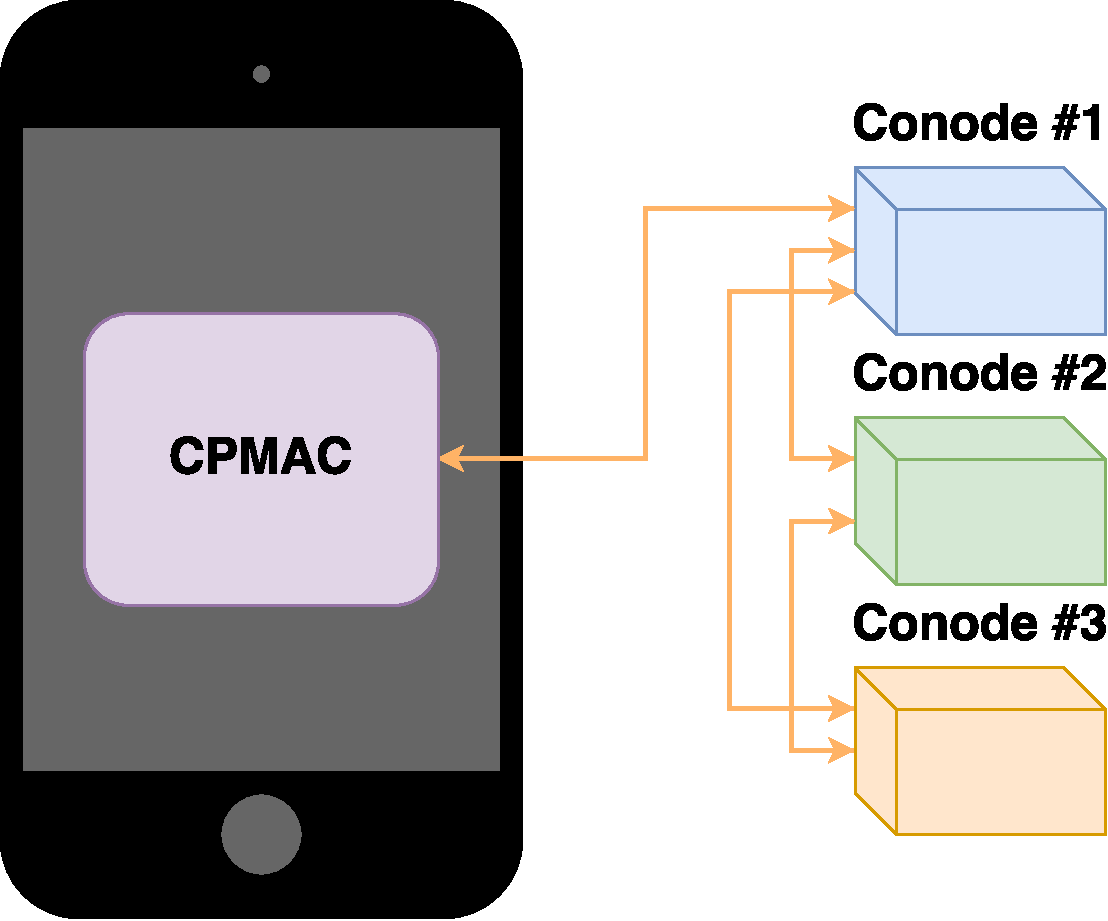
\includegraphics[scale=.5]{graphic/communication.pdf}
\centering
\caption{Inter-conode and CPMAC-conode communication.}
\end{figure}
